\documentclass{article}
\usepackage[UTF8]{ctex}  % 使用中文支持包
\usepackage[a4paper, margin=1in]{geometry}  % 设置纸张大小和边距
\usepackage{anyfontsize}  % 解决字体大小报错问题
\usepackage{fancyhdr}  % 设置页眉、页脚、页码
\usepackage{longtable}  % 支持长表格
\usepackage{booktabs} % 用于生成更好的表格
\usepackage{adjustbox} % 用于调整表格宽度

\usepackage{amsmath}  % 数学公式支持
\usepackage{cases}  % 支持联立编号
\usepackage{cite}  % 引用支持

\usepackage{graphicx}  % 插入图片支持
\usepackage{float}  % 设置图片浮动位置
\usepackage{subfigure}  % 插入多图时用子图显示

\usepackage{listings}  % 代码块支持
\usepackage{xcolor}  % 设置代码块颜色

\usepackage[hyphens]{url}  % 支持链接换行
\usepackage{hyperref}  % 超链接支持
\usepackage{lastpage}  % 添加lastpage包

\usepackage{gbt7714}  %国标参考文献

\hypersetup{
    hidelinks,
    colorlinks=true,
    allcolors=black,
    pdfstartview=Fit,
    breaklinks=true
}

\title{聚变能源概论-第八讲作业}
\author{\LaTeX\ by\ Jerry\ }
\date{\today}
\pagenumbering{arabic}

\begin{document}
\pagestyle{fancy}

\fancyhead[L]{Jerry}
\fancyhead[C]{聚变能源概论-第八讲作业}
\fancyhead[R]{\today}
\fancyfoot[C]{Page \thepage/\pageref{LastPage}}

\section*{6.2}

\emph{托卡马克利用简单、规则的线圈放电实现对等离子体的启动、约束和加热。在标准托卡马克系统中共有三类线圈,它们分别起什么作用?你能猜测三类线圈按电流大小的排序吗?为什么}

如图\ref{fig:tokamak}所示,托卡马克系统中共有三类线圈,分别是:

\begin{enumerate}
    \item 环向场线圈,它产生约束的主要磁场
    \item 欧姆场线圈,或称中心螺旋管,它通过电磁感应驱动等离子体电流以加热等离子体和产生极向磁场
    \item 外极向场线圈,或称垂直场线圈、平衡场线圈,它维持等离子体环在水平面上的平衡
\end{enumerate}

\begin{figure}[htbp]
    \centering
    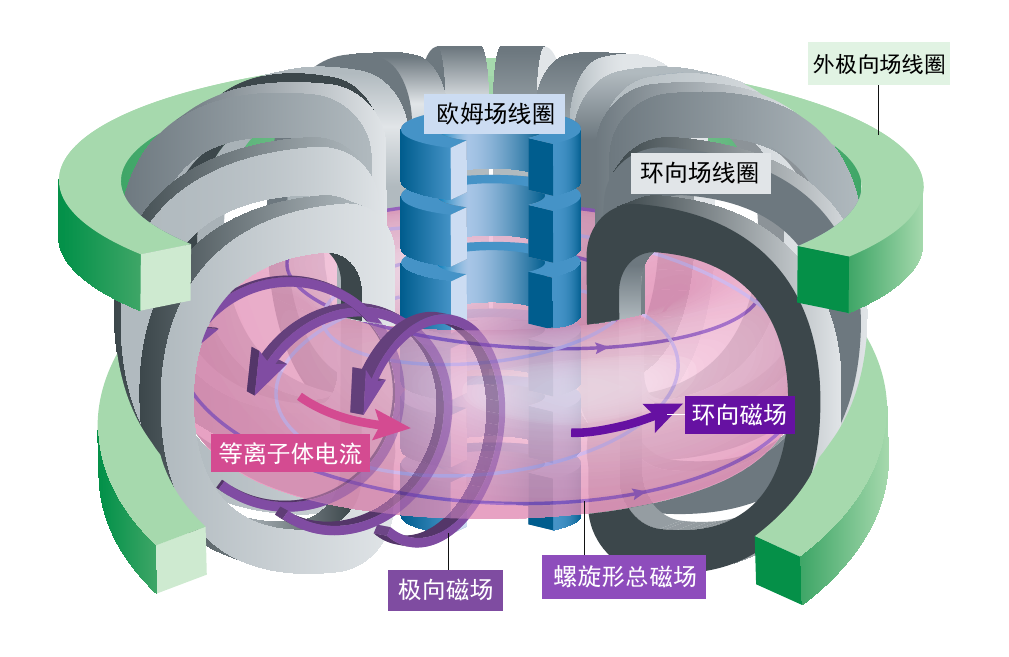
\includegraphics[width=0.8\textwidth]{img/tokamak.png}
    \caption{托卡马克示意图}
    \label{fig:tokamak}
\end{figure}

环向场线圈产生最主要的环向磁场以对等离子体形成约束,磁场最强,线圈电流最大;

磁场回转变换所需的极向磁场主要由环向等离子体电流提供,这个环向的等离子体电流一般通过电磁感应产生——这就是中心螺旋管的作用。中心螺线管磁通发生变化,在等离子体环中感应出电动势,从而驱动等离子体电流,这个电流还起到了欧姆加热、提高等离子体温度的作用。因此需要保证磁通变化量较大,需要线圈电流较小;

托卡马克的平衡首先可以理解为载流等离子体柱的径向平衡,与包含轴向磁场的𝑍箍缩等离子体柱平衡是类似的;由于载流的等离子体环会有向外膨胀的趋势,还需要垂直方向的场施加给载流等离子体一个向内的力以保持平衡,磁场最弱,所需线圈电流最小。

\section*{6.5}

\emph{阅读文章: Xu Y. A general comparison between tokamak and stellaratorplasmas[J]. Matter and Radiation at Extremes, 2016, 1(4): 192-200,比较托卡马克和仿星器的异同点,分析它们各自的优缺点。}

\begin{table}[h!]
    \centering
    \caption{托卡马克与仿星器比较}
    \label{tab:tokamak_stellarator_comparison}
    \begin{tabular}{@{}p{3cm}p{6cm}p{6cm}@{}}
    \toprule
     & \adjustbox{valign=t}{托卡马克} & \adjustbox{valign=t}{仿星器} \\
    \midrule
    磁约束配置 & 通过等离子体电流产生极化场,使磁场扭曲形成闭合曲线。托卡马克具有轴对称性,可以很好地约束碰撞粒子,但难以实现稳定的运行状态。 & 通过外部非轴对称线圈产生磁场扭曲,实现等离子体约束。仿星器天然不需要等离子体电流,因此能够保持稳定的运行状态,但存在更多未被约束的粒子轨迹。 \\
    MHD不稳定性和运行限制 & 等离子体电流会引起宏观和微观MHD不稳定性,限制了运行的可行性。需要对MHD不稳定性进行主动控制。 & 由于没有或很少的净等离子体电流,仿星器通常不存在大的MHD不稳定性,这使得仿星器能够更容易地实现稳定的运行状态。此外,仿星器在运行时也不会遇到阻断,这使得仿星器的设计更加灵活。 \\
    传输与涡流 & 在较高的等离子体温度下,传输一般较低。存在很强的离子和电子涡流效应。 & 在高温下,传输比托卡马克高。仿星器可能在较冷的部分出现湍流。 \\
    等离子体回旋 & 通常会产生较高的轴向等离子体回旋速度,这对于改善约束有帮助。 & 由于非轴对称性,回旋运动受到较大限制,且无法达到托卡马克的回旋速度。 \\
    优缺点 & 优点:技术简单、轴对称性好、低传输损耗以及较强的等离子体回旋。缺点:运行时易受MHD不稳定性影响,容易出现运行限制和中断。 & 优点:稳定运行、少MHD活动、几乎没有中断。缺点:复杂的三维磁场结构导致传输较高、设计制造复杂。 \\
    \bottomrule
    \end{tabular}
\end{table}

\section*{6.6}

\emph{阅读文章: Gao Z. Compact magnetic confinement fusion: Spherical torusand compact torus[J]. Matter and Radiation at Extremes, 2016, 1(3): 153-162,比较球形环和紧凑环的异同点,分析它们各自的优缺点}


\begin{table}[h]
    \centering
    \caption{球形环 (ST) 和紧凑环 (CT) 比较}
    \begin{tabular}{@{}lll@{}}
        \toprule
        类别 & 球形环 (ST) & 紧凑环 (CT) \\
        \midrule
        定义 & 低长宽比的托卡马克,形状接近球形 & 具有单连接几何形状的环状磁约束配置 \\
        结构 & 中心电流环 & 无通过环形等离子体中心的导体或真空室壁 \\
        \midrule
        优点 & 高 $\beta$ 值、良好的 MHD 稳定性 & 简单的连通几何形状、高 $\beta$ 值、无环形场线 \\
        \midrule
        缺点 & 非电感性启动和电流驱动难度较高 & 等离子体性能相对较低、长脉冲放电和等离子体维持困难 \\
        \bottomrule
    \end{tabular}
\end{table}

\end{document}
